\chapter{Decoding Induced Grammars}
\label{chap:decoding}


So far this report has described several techniques for inducing synchronous grammars from text and shown that some of them lead to improvements in translation quality.  Unfortunately, these improvements come at a cost: decoding with the induced grammars is more computationally expensive than decoding with the Hiero baseline grammars.  Therefore, part of the workshop was devoted to research on efficient decoding techniques for induced grammars, the focus of this chapter.

A simple example from our experimental setup illustrates the problem.  On the Urdu-English task (\textsection\ref{sec:datasets}), the baseline Hiero grammar achieves a BLEU score of 20.8, while an induced 25-category grammar scores 21.7, a substantial improvement.  However, using the same decoding algorithm, the Hiero grammar requires only 3.0 seconds to decode each sentence, while the 25-category grammar requires 52 seconds -- an order of magnitude slower.  The prospects for decoding with grammars induced from larger data using more categories are even worse.

Why is decoding so slow with these grammars?  We first answer this question from a theoretical perspective (\textsection\ref{sec:overview}), and then measure the opportunity for improvement with the help of an oracle experiment (\textsection\ref{sec:oracle}).  Finally we describe our contributions towards efficient decoding for these grammars, which include coarse-to-fine decoding (\textsection\ref{sec:ctf}) and grammar pruning techniques (\textsection\ref{sec:pruning}).

\section{Decoding with Synchronous Context-free Grammars} \label{sec:overview}

Informally, decoding with any synchronous context-free grammar is accomplished by first parsing the source sentence with the source projection of the grammar, and then reading off the string produced by the corresponding target parse.  To illustrate this, suppose that we have the following grammar.
\begin{align*}
	S &\rightarrow NP_1~VP_2 / NP_1~VP_2 \\
	NP &\rightarrow \textrm{ watashi wa } / \textrm{ I }\\
	NP &\rightarrow \textrm{ hako wo } / \textrm{ the box }\\
	VP &\rightarrow NP_1~V_2 / V_1~NP_2 \\
	V &\rightarrow \textrm{ akemasu } / \textrm{ open }
\end{align*}
We show a parse of the source sentence {\it watashi wa hako wo akemasu} under the source projection of this grammar below.\footnote{This example is borrowed from ???}  
\begin{center}
	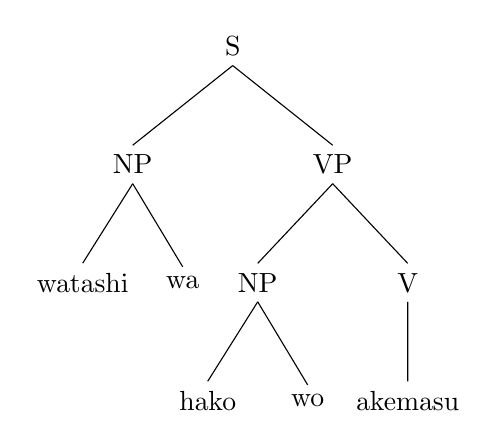
\begin{tikzpicture}[edge from parent path= {(\tikzparentnode.south) -- (\tikzchildnode.north)}]
		\node{S}[sibling distance=1in]
			child {node {NP}[sibling distance=0.5in]
				child {node {watashi}}
				child {node {wa}}}
			child {node {VP}[sibling distance=0.75in]
				child {node {NP}[sibling distance=0.5in]
					child {node {hako}}
					child {node {wo}}}
				child {node {V}
					child {node {akemasu}}}};
	\end{tikzpicture}
\end{center}
This parse implies a corresponding unique target parse tree that is isomporphic to the source parse up to the ordering of child nonterminals and the identity and ordering of nonterminals, as illustrated below.  All that is needed to obtain the translation is to read off the target nonterminal string at the leaves of the tree.  
\begin{center}
	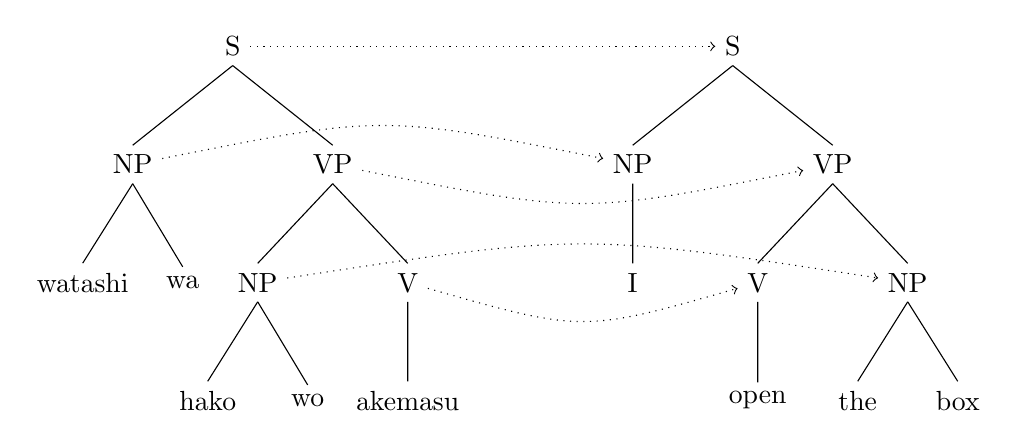
\begin{tikzpicture}[edge from parent path= {(\tikzparentnode.south) -- (\tikzchildnode.north)}]
		\node(S1a) at (0,0){S}[sibling distance=1in]
			child {node(NP2a) {NP}[sibling distance=0.5in]
				child {node {watashi}}
				child {node {wa}}}
			child {node(VP3a) {VP}[sibling distance=0.75in]
				child {node (NP4a) {NP}[sibling distance=0.5in]
					child {node {hako}}
					child {node {wo}}}
				child {node(V5a) {V}
					child {node {akemasu}}}};
		\node (S1b) at (2.5in,0) {S}[sibling distance=1in]
			child {node (NP2b) {NP}[sibling distance=0.5in]
				child {node {I}}}
			child {node (VP3b) {VP}[sibling distance=0.75in]
				child {node (V5b) {V}
					child {node {open}}}
				child {node (NP4b) {NP}[sibling distance=0.5in]
					child {node {the}}
					child {node {box}}}};
		\draw[->,dotted] (S1a) -- (S1b);
		\draw[->,dotted] (NP2a) ..controls +(1.25in,0.25in) .. (NP2b);
		\draw[->,dotted] (VP3a) ..controls +(1.25in,-0.25in) .. (VP3b);
		\draw[->,dotted] (NP4a) ..controls +(1.625in,0.25in) .. (NP4b);
		\draw[->,dotted] (V5a) ..controls +(0.875in,-0.25in) .. (V5b);
	\end{tikzpicture}
\end{center}
In general, however, there will be more than one parse of a given sentence -- indeed, there may be exponentially many parses.  The set of all possible parses can can be computed efficiently using dynamic programming in the form of the CKY algorithm or its variants (we use CKY+).  This produces a {\it hypergraph} (or {\it packed chart}) containing all parses, which requires at most $O(Gn^3)$ time to construct.  The value $G$ is a grammar constant tied to properties of the grammar -- as a loose bound, it will be at least cubic in the size of the set of nonterminal symbols.  Consequently, a key problem is that {\bf parsing time is strongly correlated with the number of nonterminal symbols in the grammar}.  This is why parsing with 25 categories is an order of magnitude slower than parsing with two categories as in the baseline.

Of course, parsing the source does not completely solve the translation problem, as in our translation models we need to consider the probability of each string under an $n$-gram language model.  This intersection carries with it even worse computational overhead.  A common approach to decoding with synchronous grammars is the {\it two-pass} strategy.
\begin{enumerate}
	\item The source sentence is {\it exhaustively} parsed to produce a packed chart (called the {\it -LM hypergraph}).
	\item This chart, itself a context-free grammar encoding all possible target sentences, is then intersected with an $n$-gram language model.  The search space for this intersection is a much larger hypergraph (called the {\it +LM hypergraph}), constructed with heavy pruning to counteract complexity effects.
\end{enumerate}
Although some algorithms in the literature are only described implicitly in these terms, most of them follow this strategy \citep{Chiang2005,Huang+Chiang:2007:acl,venugopal-zollmann-stephan:2007:main,denero-EtAl:2009:NAACLHLT09,denero-pauls-klein:2009:Short,hopkins-langmead:2009:EMNLP,hopkins-langmead:2010:EMNLP,iglesias-EtAl:2009:NAACLHLT09}.  The most popular of these, the {\it cube pruning} algorithm of \citet{Chiang2005}, is the baseline algorithm implemented in our decoder \citep{dyer-EtAl:2010:Demos}, making it a natural starting point for our exploration.  The amount of work done in cube pruning is a constant multiplier times the size of the -LM hypergraph, so reducing its size is the key to producing faster two-pass algorithms.  Therefore, we will consider approaches that construct a pruned -LM hypergraph.

\section{Oracle Experiments}\label{sec:oracle}

At the outset, we wondered what effect substituting a pruned -LM hypergraph for the full -LM hypergraph would have on translation accuracy.  To measure this, we ran an oracle experiment.  
\begin{enumerate}
	\item Produce the complete -LM hypergraph.
	\item Prune the -LM hypergraph using inside-outside pruning.
	\item Integrate the language model on the pruned -LM hypergraph via cube pruning.
\end{enumerate}
The idea behind inside-outside pruning is simple: since we have access to the complete chart, we can calculate the ratio between the globally highest-scoring parse and the highest-scoring parse passing through any particular hyperedge.  We prune the hyperedge if this ratio falls below some pruning threshold.  By varying the threshold, we retain -LM hypergraphs of different sizes.

An important point is that the -LM hypergraph incorporates only local features from the translation model and not the non-local language model feature.  This has two consequences.  First, it is possible to prune away the parse yielding the globally optimal translation under the combined model.  Second, the ranking of parses under the translation model features is likely to be very poor.  Nonetheless, it is important to recognize that the experiment is still idealized because it incorporates information from the full -LM hypergraph during pruning, and this information will not be available to us in practical methods that must avoid building the full -LM hypergraph altogether.

The results of an initial oracle experiment are shown in Figure~\ref{figure:oracle-untuned}.  These initial results are discouraging: we find that it is only possible to prune between twenty and thirty percent of the -LM hypergraph without incurring penalties in downstream BLEU score.

\begin{figure}
	\includegraphics[scale=0.5]{prune-untuned}
	\caption{Oracle experiment: final BLEU score vs. percent of -LM forest retained after an initial inside-outside pruning pass. \label{figure:oracle-untuned}}
\end{figure}

This initial result was disappointing, so we considered a different oracle approximation.  In this case, we first tuned the local features using minimum error rate training, and used the subsequent set of feature weights for inside-outside pruning.  This approximation turns out to produce a much better inside-outside pruning of the first-pass hypergraph.  The results  show (Figure~\ref{figure:oracle-tuned}) that it is possible to discard much more of this hypergraph before the second pass without harming overall accuracy -- possibly as much as three quarters of it.  This result shows that heavy pruning of a -LM forest might be a means of improving decoding speed without harming translation accuracy.

\begin{figure}
	\includegraphics[scale=0.5]{prune-tuned}
	\caption{Second oracle experiment: final BLEU score vs. percent of -LM forest retained after an initial inside-outside pruning pass using weights tuned for -LM decoding. \label{figure:oracle-untuned}}
\end{figure}

\section{Coarse-to-Fine Decoding}\label{sec:ctf}

Motivated by our oracle experiment, we implemented {\it coarse-to-fine parsing} to generate the -LM hypergraph.  The idea behind the algorithm is simple: we first parse the source sentence using a projected grammar with a much lower grammar constant (the coarse grammar), which can be done very quickly.  The resulting hypergraph is pruned using inside-outside, and we then parse the sentence again with the true grammar (the fine grammar), limiting the parse only to those edges whose projection appears in the pruned coarse hypergraph.  If the original parse is sufficiently pruned, then this second pass will take much less time than an exhaustive parse with the same grammar.

The first decision we need to make is how to obtain the coarse grammar.  Many strategies are possible; for our experiments we chose to simply map all nonterminals to X.  In essence, this means that we are decoding with the baseline Hiero grammar; although \citet{denero-EtAl:2009:NAACLHLT09} found that this simple strategy was ineffective for grammars estimated using parsers, the strategy makes intuitive sense for our induced grammars since they are generated by decorating Hiero grammars with finer-grained categories.  As shown in Figure~\ref{fig:ctf}, we found that by varying the pruning parameter, we obtained different tradeoffs in speed and accuracy.  Most encouraging, however, was the fact that we were able to lower decoding speed by nearly 40\% without any reduction in overall translation accuracy.

An implementation detail that was important to our experiments was re-parsing.  A subtle feature of coarse-to-fine parsing is that some coarse parses do not correspond to any parse in the fine grammar -- this is a consequence of the coarse grammar conflating two otherwise distinct nonterminal symbols.  We discovered that a fairly common failure case for our parser occurred when all coarse parses corresponding to true fine parses were pruned away in the first pass.  To work around this problem, whenever a fine parse was not found, we widened the beam and repruned the coarse hypergraph more conservatively.

\section{Grammar Pruning}\label{sec:pruning}

An alternative means of reducing the overhead of parsing is to prune the translation grammar.  Although a pruned grammar will still retain the same number of nonterminal symbols, parsing time may be substantially improved if there are simply fewer 

\section{Discussion}





